\cotefile{156-3}
\scanpage{10}\mspage{9}
% ink top, lines 1–3
un \uline{demi}-\uline{intervalle} s'il admet un plus petit \unsure{élément} mais pas un plus grand, ou bien l'inverse.

% ink upper middle, NB, lines 1–4
\deleted{\unsure{L'opposé|L'oppo}}\inserted{\uline{NB}} L'opposé d'un tronçon, segment, intervalle, demi-intervalle est itou. L'opposé d'un $1/2$ intervalle fermé à g. est fermé à droite, et \unsure{inversement}.
% ink left, slanting upwards beside NB
% slanted
\margin{Dans \unsure{ma|sa} \unsure{actuelle|initiale} \unsure{terminologie}, tronçon \unsure{est|être|était|etre} \unsure{``ens|ens|un|équiv} \uline{\unsure{biordre|biordonné}}}

% ink middle, Tout, lines 1–3
\deleted{\unsure{Lorsque|Lorsqu.}}\inserted{Tout} tronçon est l'un des trois (segment, $1/2$ intervalle, intervalle) à l'exclusion \unsure{des} deux autres.

% ink lower middle, Si L
Si $\mathcal L$ est un tronçon, on pose $\deleted{\unsure{\partial L}=}$
\[
\begin{aligned}
\unsure{\partial L|\partial}&=\bigl\{\,x\in L\mid
\begin{aligned}&x\text{ est plus petit élément}\\
&\text{ou plus grand \unsure{élément|élt}}\end{aligned}\,\bigr\}
\end{aligned}
\]
\deleted{\illegible{1}}

% ink bottom, Soit and first equality
Soit $\mathcal L$ un tronçon, et
\[
\begin{aligned}
\unsure{\mathscr S|S}_0(L)=\mathrm{Drap}_2(L)&=\{\,\unsure{E|\mathcal E}\in\unsure{\mathrm P|\mathscr P}_2(L)\mid E\text{ tot ordonné}\,\}\\
&=\{\,\{x,y\}\mid x<y\,\}
\end{aligned}
\]
% ink bottom, final equality
\[
\text{D'où}\qquad \unsure{\mathrm{Modf}|\mathrm{Mod}_{f}}(L)=\mathrm{Drap}(L)
=\{\,S\subset\mathrm P_f(L)\mid S\,\substack{\text{tot}\\\text{ord}}\,\}
\]
\scanpage{11}\mspage{10}
% ink top, Si S and C(S)
Si $S\in\unsure{\mathrm{Modf}|\mathrm{Mod}_{f}}(L)$, on a donc $\deleted{C(S)=}$
\[
C(S)=\{\,\deleted{\unsure{s|x}}t\in L\mid\deleted{\unsure{S\cup\{t\}}}\ t\notin S,\quad S\cup\{t\}\ \text{tot. ord}\,\}
\]

% ink upper third, On a dit
On a dit comment on décomposait en ``composantes connexes'' un $C(S)$ \unsure{où|à|.}
\[
 S=\{s_{\deleted{\unsure{0}}1},\ldots s_n\},\qquad s_{\deleted{\unsure{0}}1}<s_2,\!<\cdots<s_n\,.
\]
Les comp. connexes sont les ens non vides parmi
\[
L_{<s_{\deleted{\unsure{0}}1}},\quad \deleted{\unsure{L}}[s_{\deleted{\unsure{0}}1},s_2],\quad\ldots,\ [s_{n-1},s_n],\quad L_{>s_n}
\]
% ink middle, bracketed cases
\[
\begin{aligned}
\bigl[\quad&\text{cas }n=0:\quad\text{une seule comp. }\mathcal L\\
&\text{\unsure{cas|en} }n=1:\quad\deleted{\text{\unsure{une}}}\ \text{deux composantes}\quad L_{<s},\ L_{>s}\\
&\hspace{7em}\text{(celles qui sont non vides)}\\
&\text{cas }n\geq2:\quad\text{voir \unsure{la|le|ce} \unsure{suite|suit} plus haut}\quad\bigr]
\end{aligned}
\]
% ink below cases, two extreme components
les seules non vides \unsure{éventuelles} étant $L_{<s_1}$ (\inserted{si} $s_1$ plus petit élément) et $L_{>s_n}$ (\inserted{si} $s_n$ \unsure{plus grd} élément). Les bords \deleted{sont} respectivement
% ink lower third, bords
\[
\underset{\substack{\rule{.4pt}{.6ex}\rule{4.8em}{.4pt}\rule{.4pt}{.6ex}\\\text{si comp. existe}}}{\{s_1\}\ \substack{\deleted{\unsure{s_1}}\\\deleted{\unsure{\text{donc }\varnothing}}\\\deleted{\unsure{\varnothing}}}},
\quad\{s_1,s_2\},\quad\ldots,\quad\{s_{n-1},s_n\},\quad
\underset{\substack{\rule{.4pt}{.6ex}\rule{2.7em}{.4pt}\rule{.4pt}{.6ex}\\\text{si comp. existe}}}{\{s_n\}}
\]

% ink bottom, Je dis
Je dis que l'on récupère la structure \unsure{dé|de} \deleted{\unsure{ordr|ordre}} biordre du tronçon (donc aussi \unsure{les structures|la structure} \textcircled{a}\unsure{.} \textcircled{b} \textcircled{c}) en termes de la seule structure \textcircled{a}, $+$ \textcircled{b} pour $T\in\unsure{\mathscr S|S}_0$.
\scanpage{12}\mspage{11}
% ink opening line
Pour ceci, on note \deleted{\unsure{qu'une str}}\inserted{d'abord}

% ink Lemme, first four lines
\uline{Lemme} Une structure de \deleted{biordre} tronçon \unsure{biordonnien|biordonnier} est connue quand on connaît la relation en \deleted{$\{a,b,c\}$} trois \unsure{élémt|éléments} $a,b,c$
% ink relation R, first display
\[
\begin{aligned}
\left.\vphantom{\substack{X\\X}}\right|\!\left.\vphantom{\substack{X\\X}}\right|\!\left.\vphantom{\substack{X\\X}}\right|\, R(a,b,c)
&\qquad b\ \text{\uline{est strictement entre}}\\
&\qquad\qquad\text{\uline{$a$ et $c$}}
\end{aligned}
\]
(au sens que $a<b<\deleted{\unsure{e}}c$ \uline{ou} $a>b>c$)
% ink left, short diagonal note beside the three strokes
% slanted
\margin{relation sym. en $a,c$}
% ink left, NB, diagonal block
% slanted
\margin{\uline{NB} \deleted{\unsure{On a de}}\inserted{La \unsure{conn.} de} \unsure{Cette|cette} relation $R$ implique la relation $\bar R$ non stricte \deleted{\unsure{($a=b=c$} \unsure{ou}}\ \deleted{$\unsure{a=b<c}$}\ $a\leq b\leq c$ ou $a\geq b\geq c$ \deleted{$\unsure{a\leq b\leq c}$} \deleted{$(\unsure{\Leftrightarrow})$} \deleted{$\{a,b,c\}$} $b$ entre $a$ et $c$ \inserted{\uline{strict}} ou $\{a,b,c\}$ est un drapeau de cardinal $\leq 2$}

% ink middle, Dém and équivalence
\uline{\unsure{Dém|Dém.}} \deleted{Choisissons} On en déduit la relation (i.e. \inserted{la \unsure{conn.} de} $\unsure{\mathscr S|S}_0(L)$\deleted{\unsure{)}} i.e. de $\mathrm{Drap}(L)$)
\[
\begin{aligned}
\deleted{\unsure{a}}\,a\text{ et }b\ \text{``disjoints''}\quad&
\text{i.e. distincts et comparables}\\
&\text{(i.e. }\{a,b\}\in\mathrm{Drap}_2(L)\\
&\text{pour le biordre}
\end{aligned}
\]
% ink lower middle, formule ssi
\unsure{par|puis|pour} 
\[
\begin{aligned}
a\text{ et }b\ \text{\unsure{disjts}}\quad \text{ssi}\quad
\exists\,c\ \text{tel que }c\text{ entre}\\
a\text{ et }b
\end{aligned}
\]
(utilise \unsure{divisibilité !} d\deleted{\unsure{es}}\unsure{u} \deleted{\unsure{drap. le ré}} biordre)

% ink bottom, Choisissons
\deleted{\illegible{1}} Choisissons $\unsure{E|\mathcal E}\in\mathscr S_0$ (existe, car \deleted{si $x,y\in$} par \unsure{hyp} $\exists\,x,y\in L,\quad x\ne y$, donc $a\leq x,y\leq b$, et on a $a\leq b$ et $a\ne b$ \deleted{\unsure{)}} \deleted{\unsure{c|p}}\unsure{car} sinon on \unsure{aurait} $x=y$)
% ink lower left, four short oblique lines
% slanted
\margin{\unsure{Il} existe $=$ des \unsure{drap.} de \unsure{long.} arbitraire}
\scanpage{13}\mspage{12\unsure{..|.}}
% ink top, first two lines
\unsure{et|Et} choisissons une ``origine'' $a$ dans $\unsure{E|\mathcal E}=\{a,b\}$ (ce qui va déterminer la relation d'ordre).

% ink upper third, Considérons
\deleted{Soit} \deleted{Alors} Considérons sur $\mathcal L$ la relation d'ordre \unsure{définissant} le biordre, telle que $a<b$. On va voir qu'elle est \unsure{entièmt|entièrement} \unsure{déterminée} par la conn. \deleted{\unsure{de}}\unsure{du} \deleted{\unsure{la paire}}\inserted{couple} $(a,b)$

% ink upper middle, On aura, three defining sets
On \unsure{aura|a} \unsure{.}
% slanted
\margin{déterminés par $R$}
\[
\left\{\begin{aligned}
\mathcal L_{\deleted{\unsure{>}}\geq b}&=\{\,x\in L\mid\deleted{x=b\text{ ou}}\ \inserted{x=b\text{ ou}}\ b\text{ entre }a\text{ et }x\,\}\quad\deleted{\unsure{a,b|a<b}.}\\
\mathcal L_{\leq a}&=\{\,x\in L\mid\inserted{x=a\text{ ou}}\ a\text{ entre }\deleted{\unsure{a}}b\text{ et }x\,\}\\
\deleted{\unsure{\mathcal L}}\mathopen{]}\deleted{\unsure{x}}a,b\mathclose{[}&=\{\,x\in L\mid x\text{ entre }a\text{ et }b\,\}
\end{aligned}\right.
\]
% ink left, below brace
% slanted
\margin{\unsure{donc}}

% ink middle, question
\deleted{Quand}\inserted{Soient} $u,v\in L$, quand a-t-on
\[
u\leq v\qquad\unsure{\mathord{?}|.}
\]
Il faut et suffit qu'il existe
\[
\begin{aligned}
&\deleted{x\in}\quad x,y\in L\quad\text{tels que}\\
&x\in L_{\leq a},\ y\in L_{\geq b}\qquad\text{et}\\
&\hspace{2em}x\leq u\leq v\leq y
\end{aligned}
\]
% ink bottom, i.e., left bracket
\[
\text{i.e.}\quad
\left[\begin{aligned}
&\deleted{\{\unsure{x},y,\unsure{u|b},v\}\ \text{est }\in\mathrm{Drap}(\mathcal L)}\\
&\qquad\deleted{x,y\in}\quad x\in L_{\leq a},\ y\in L_{\geq b}\quad(\text{donc }x\unsure{<|\leq}y)\\
&\deleted{\text{avec }x\text{ plus petit élément}}\\
&\deleted{u\text{ est entre}}\quad u,v\text{ sont entre }x\text{ et }y\\
&\quad u\text{ est entre }x\text{ et }v\qquad\unsure{.}\\
&\quad v\text{ est entre }u\text{ et }y
\end{aligned}\right.
\]
\scanpage{14}\mspage{13}
% ink top, opening and lemma
Donc il faut simplement vérifier le

\uline{Lemme} Soit $\mathcal L$ un ens ordonné, et $x,y,u,v$ trois \unsure{élémts|éléments}, tels que
% ink upper third, clauses a–d and brace at right
\[
\begin{aligned}
&\text{a)}\quad u,v\text{ sont entre }x\text{ et }y\\
&\left.\begin{aligned}
&\text{b)}\quad u\text{ est entre }x\text{ et }v\\
&\unsure{(}[\,\text{c)}\quad v\text{ est entre }u\text{ et }y\,]\deleted{\unsure{)}}
\end{aligned}\ \right\}\quad
\begin{aligned}&\text{une des deux}\\&\text{\unsure{en} suffit}\end{aligned}\\
&\text{d)}\quad x<y\quad,
\end{aligned}
\]
alors on a
\[
x\leq u\leq v\leq y
\]

% ink middle, Dém, first four lines
\uline{\unsure{Dém|Dém.}} \deleted{\unsure{L'ass|L'assert}} \unsure{les|Les} conditions b)\unsure{,} c) d) impliquent que $I\deleted{\unsure{\{x}}=\{x,y,u,v\}$ est un drapeau, \deleted{\unsure{Prouvons|Prenons}} et \unsure{SPG} $\mathcal L=I$ est un ens tot. ordonné \deleted{que $x$ en} à 2, 3, ou 4 \unsure{élémts|éléments}.
% ink middle, crossed proof and interlinear replacement
\deleted{Alors \unsure{Prouvons|Prenons}} \inserted{Comme $u,v$ sont} \deleted{que $x$ est le plus petit élément, donc (comme $x<y$) que l'on ne peut avoir $u<x$, ni $v<x$. \unsure{Supposons} $u<x$ ($<y$) ; comme $u$ est entre $x$ et $v$, on aurait \unsure{$v\leq u<$}\ $v<u<x<y$} \inserted{entre $x$ et $y$ et $x<y$,} on doit avoir $x\leq u,v\leq y$, \deleted{il reste à prouver $u\leq v$} et comme $u$ est entre $x$ et $v$, on doit avoir $x\leq u\leq v$\quad OK

% ink bottom, NB and lettered lines
\uline{NB} On a utilisé
\[
\begin{aligned}
&\text{a) la divisibilité de la \unsure{rel.} d'ordre}\\
&\text{b) le fait que }\mathcal L\text{ soit \unsure{filtrant}}\\
&\hspace{2em}\text{\unsure{croissant} et filtrant \unsure{décroissant}.}
\end{aligned}
\]
% ink last two lines
Et a) n'a servi qu'à montrer que la relation ``$a$ et $b$ disjoints'' est déductible de ``$a$ est str. entre $b$ et $c$''
\scanpage{15}\mspage{14}
% ink top, relations
Si on se donne à la fois les deux relations
\[
\left\{\begin{aligned}
\unsure{\underline R|R}(a,b)&\qquad \{a,b\}\in\mathrm{Drap}_2(L)\\
R(a,b,c)&\qquad b\text{ est str. entre }a\text{ et }c
\end{aligned}\right.
\]
alors pour \unsure{récupérer} le biordre, il suffit de supposer $\mathcal L$ filtrant croissant et filtrant décroissant, \deleted{et les relations \unsure{Si|si}, \unsure{Cet|cet|Oct} \unsure{sur les}, filtrant \unsure{cr.} et \unsure{décr.} \unsure{sont} de \unsure{qque|toutes} \unsure{comp.|faç.} \unsure{connexes|connues en} \unsure{$S_0$|$v_0$|$0$}} 

% ink middle, On va voir
\deleted{\unsure{On va}} On va voir maintenant comment la connaissance\inserted{ de $\mathrm{Drap}_2(L)$, et} pour $\unsure{E|\mathcal E}\in\mathrm{Drap}_2(\deleted{\unsure{I}}L)$, de la \unsure{décomp.} de
% ink middle, C(E) and continuation
\[
 C(E)=\{\,t\in L\deleted{\unsure{\notin E|\smallsetminus E}}\mid
 \deleted{\unsure{x}}\{E\unsure{\cup|,}t\}\deleted{\unsure{=|-}}\in\mathrm{Drap}_3(L)\,\}
\]
en composantes connexes, implique la connaissance de la relation
\[
 R(a,b,c)\unsure{\mathord{:}|\mathord{?}}\quad b\text{ strict entre }a\text{ et }c.
\]
% ink lower third, Première condition
\unsure{Première} condition : $\{a,b,c\}\in\mathrm{Drap}_3(L)$ (\unsure{résulte} de la donnée de $\mathrm{Drap}_2(L)$)
\figure{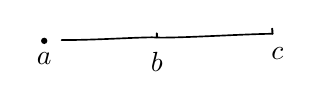
\begin{tikzpicture}[x=1cm,y=1cm,line cap=round]
\fill (0,0) circle (1.15pt);
\draw[line width=.6pt] (.22,.01) .. controls (.66,.01) and (1.06,.04) .. (1.37,.045) .. controls (1.61,.026) and (2.48,.085) .. (2.9,.09);
\draw[line width=.7pt] (1.43,.045) -- (1.43,.095) (2.9,.09) -- (2.895,.155);
\node[below] at (0,-.025) {$a$};
\node[below] at (1.43,-.015) {$b$};
\node[below] at (2.96,.035) {$c$};
\end{tikzpicture}}
% ink bottom, final sentence and cancelled display
Si $b$ est entre $a$ et $c$, regardons les
\[
 \deleted{\unsure{J|I}_{abc}=\text{composante de }C(\{a,b\}}\unsure{,|)}
\]
\scanpage{16}\mspage{15}
% ink top, heading of the three equalities
trois composantes (relatives à la \unsure{donné|donnée} de $\{a,b,c\}$)
\[
\begin{aligned}
\deleted{\unsure{C}}X_{\{a,b\}}&=\deleted{\unsure{C(a,b,c)}}=(\text{comp. de }C(\{a,b\})\text{ contenant }c)=L_{>b}\\
X_{\{b,c\}}\deleted{\unsure{C(b,c,a)}}&=(\rule{1.45cm}{.4pt}\ C(\{b,c\})\ \rule{1.1cm}{.4pt}\ a)=L_{<b}\\
X_{\{c,a\}}\deleted{C(c,a,b)}&=\rule{1.2cm}{.4pt}\ C(\{c,a\})\ \rule{.85cm}{.4pt}\ b)=\deleted{\unsure{\mathcal L}}\mathopen{]}a,c\mathclose{[}
\end{aligned}
\]

% ink middle, On trouve and three intersections
On trouve
\[
\begin{aligned}
&\deleted{C}X_{\{a,b\}\deleted{\unsure{c}}}\cap\deleted{C}X_{\{b,c\}\deleted{\unsure{a}}}=\varnothing\\
&\left.\begin{aligned}
&\deleted{C}X_{\{a,b\}\deleted{\unsure{c}}}\cap\deleted{C}X_{\{c,\deleted{\unsure{b}}a\}\deleted{\unsure{b}}}=\mathopen{]}b,c\mathclose{[}\ne\varnothing\\
&X_{\unsure{(\,|\,\{}b,\unsure{c|b}\}}\cap X_{\{c,a\}}=\mathopen{]}a,b\mathclose{[}\ne\varnothing
\end{aligned}\right\}
\end{aligned}
\]
% ink right of the two nonempty intersections
\margin{divisibilité !}
% ink lower middle, donc b
donc $b$ est distingué, dans $J=\{a,b,c\}$, par la propriété que pour les deux \deleted{\unsure{parties}} ${\unsure{E|\mathcal E|\varepsilon}}',E'$ \deleted{de} $\in\unsure{\mathrm P|\mathscr P}_2(J)$ qui le \unsure{contient|contiennent}, on a
\[
 X_{\unsure{E_{0}|E_{,}|E}}\unsure{\wedge|\cap}X_{E'}=\varnothing\,.\qquad\text{On gagne !}
\]

% ink bottom, NB
\uline{NB} On a à nouveau utilisé la divisibilité.
\scanpage{17}\mspage{16}
% ink heading and first remark
\uline{Remarques} \textcircled{1} \deleted{\unsure{Considér|Considé}} sur la notion de tronçon. On cherche une sous-cat. pleine \inserted{$\unsure{\mathscr T|\mathcal T}$} de celle des ens. ordonnés, satisfaisant

% ink item a, two lines and qualification at the right
a) \deleted{\unsure{S}}Tout $\mathcal L\in\mathrm{Ob}\,\mathscr T$ est filtrant croissant et filtrant décroissant, et \deleted{non vide} \inserted{de cardinal $\ne1$} (donc $\geq2$)

% ink item b
b) Si $x,y\in\deleted{\unsure{T}}\mathcal L_{\deleted{\unsure{,|g}}}\in\deleted{\unsure{O}}\mathrm{Ob}\,\mathscr T$, et $x<y$, $\exists$
\[
 z\in L,\qquad x<z<y\qquad\text{(divisibilité)}
\]

% ink item c
c) Si $x\in L\in\unsure{\mathrm{Ob}|\mathrm D}\,\mathscr T$, \deleted{alors} et si
\[
 L_{>x}\ne\varnothing,\quad\text{alors}\quad L_{>x}\in\mathrm{Ob}\,\mathscr T\,.
\]

% ink item c prime
c$'$) Dual de c)

% ink middle and lower third, Il y a
Il y a une plus grande $\mathscr T$ qui satisfait ces conditions, et $\mathscr T$ est stable par passage à l'ordre opposé. Les objets de $\mathscr T$ sont les tronçons \unsure{ordonnés}.

% ink bottom, second remark
\textcircled{2} Il faudrait expliciter \unsure{quelle|quelles} \unsure{condition|conditions} la relation $R(a,b,c)$ doit satisfaire, pour définir une structure de tronçon \unsure{biordonné|biordonnien}\unsure{,} et itou pour la donnée de $\unsure{\mathscr S|S}_0\subset\unsure{\mathrm P|\mathscr P}_2(L)$ et les $R_{\unsure{E|\mathcal E}}$\unsure{,} ($E\in\mathscr S_0$) sur les $C(E)$ \ldots
